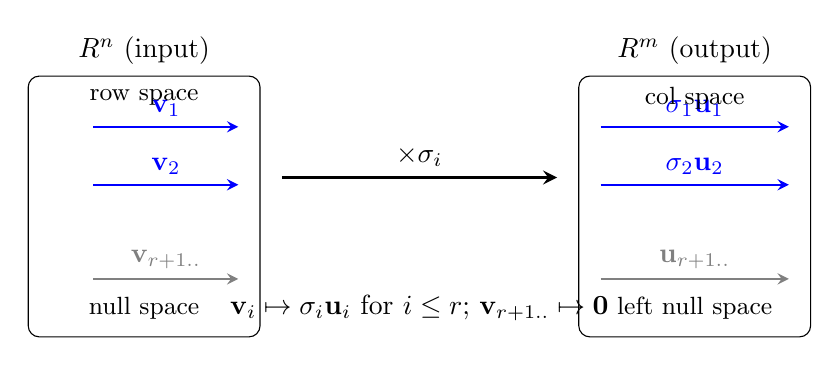
\begin{tikzpicture}[scale=0.92,>=stealth]
% V side -> sigma -> U side with four-subspace labels
\draw[rounded corners] (-0.6,-1.4) rectangle (2.6,2.2);
\draw[rounded corners] (7.0,-1.4) rectangle (10.2,2.2);
\node at (1.0,2.55) {$\mathbb R^n$ (input)};
\node at (8.6,2.55) {$\mathbb R^m$ (output)};
\draw[->,thick,blue] (0.3,1.5)--(2.3,1.5) node[midway,above]{$\mathbf v_1$};
\draw[->,thick,blue] (0.3,0.7)--(2.3,0.7) node[midway,above]{$\mathbf v_2$};
\draw[->,thick,gray] (0.3,-0.6)--(2.3,-0.6) node[midway,above]{$\mathbf v_{r+1..}$};
\node at (1.0,1.9) {\small row space};
\node at (1.0,-1.0) {\small null space};
\draw[->,very thick] (2.9,0.8)--(6.7,0.8) node[midway,above]{$\times\sigma_i$};
\draw[->,thick,blue] (7.3,1.5)--(9.9,1.5) node[midway,above]{$\sigma_1\mathbf u_1$};
\draw[->,thick,blue] (7.3,0.7)--(9.9,0.7) node[midway,above]{$\sigma_2\mathbf u_2$};
\draw[->,thick,gray] (7.3,-0.6)--(9.9,-0.6) node[midway,above]{$\mathbf u_{r+1..}$};
\node at (8.6,1.9) {\small col space};
\node at (8.6,-1.0) {\small left null space};
\node at (4.8,-1.0) {$\mathbf v_i\mapsto\sigma_i\mathbf u_i$ for $i\le r$; $\mathbf v_{r+1..}\mapsto\mathbf0$};
\end{tikzpicture}
